% !TeX root = ../main.tex

\chapter{水下穿戴式感知增强系统设计}
[总体介绍大约500字:将下面的语言再结合防水,可靠,有效性等方面进行描述扩展]
潜水员在深海环境中工作面临着复杂的水下环境。为了帮助潜水员在水下作业时提供全面的外界感知,
本章设计了一套具备水下环境三维可视化渲染功能的可穿戴系统。
该系统基于水下图像增强算法和三维重建技术,能够高质量恢复水下图像,并结合3D高斯泼溅技术渲染出逼真的水下场景。
通过嵌入手势识别技术,系统实现了人机交互功能,为潜水员在复杂场景下提供直观的视觉增强和操作便利性。

\section{系统平台搭建} 
\subsection{硬件选型与系统架构}
本章设计的水下穿戴式感知增强系统主要由相机、头戴式显示器、嵌入式处理器以及电源模块组成,
如图\ref{img:system}所示。
\begin{figure}
    \centering
    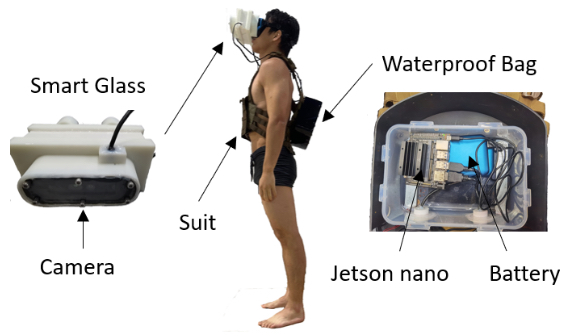
\includegraphics[width=0.8\textwidth]{figures/ch5/architecture of system.jpg}
    \caption{水下穿戴式感知增强系统组成}
    \label{img:system}
\end{figure}

(1)相机:
选用Realsense D455作为主摄像头,具备RGB-D功能,能够同时采集高分辨率的彩色图像和深度信息。
该相机封装于丙烯酸材料制成的防水外壳内,保证在水下高压环境中的稳定性。
其分辨率达到1280x720,帧率可达90fps,能够实时提供清晰的环境信息。

(2)头戴式显示器:
头显采用5英寸显示屏,分辨率为1920x1080像素,确保潜水员可以清晰地查看相机捕获的图像和三维场景。
显示器通过微型HDMI与嵌入式计算机连接,外壳基于谷歌VR纸板设计并用环氧树脂进行防水处理,确保水下使用的可靠性。

(3)嵌入式处理器:
选用NVIDIA Jetson Orin Nano作为核心计算单元,具备强大的边缘计算能力。
其GPU架构为Ampere,拥有48 Tensor Cores,支持深度学习推理加速,能够实时处理去噪扩散模型和3D高斯泼溅算法所需的计算任务。
处理器支持10W和20W两种功耗模式,结合自适应供电机制,确保系统在高性能和低功耗之间平衡。

(4)电源模块:
系统采用高容量锂电池组,容量为20,000mAh,输出电压为12V,满足Jetson Orin Nano的电力需求。
电池组集成于防水背包中,通过防水接头连接处理器,具备充电和过载保护功能,确保长时间潜水作业的稳定运行。

\subsection{防水与机械设计}
在水下环境中,设备的防水性和结构强度是决定系统可靠性的重要因素。
本系统设计了一套集成化的防水舱体与结构优化方案:

(1)防水背包:
\begin{figure}
    \centering
    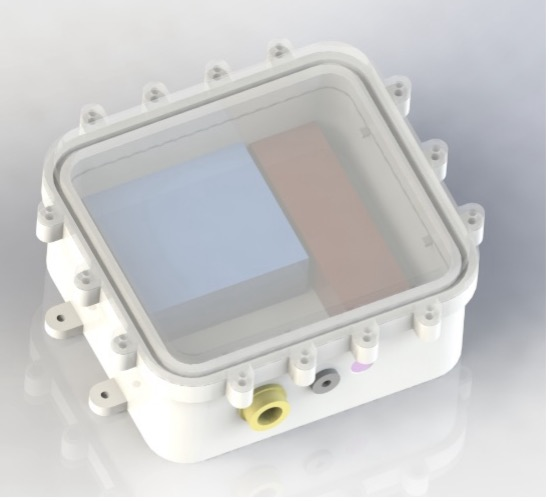
\includegraphics[width=0.8\textwidth]{figures/ch5/bag.jpg}
    \caption{防水背包设计}
    \label{img:bag}
\end{figure}

如图\ref{img:bag}所示,背包外壳采用高强度工程塑料,表面涂覆抗腐蚀层。
密封方式采用多层硅胶垫片与不锈钢紧固件结合,确保防水等级达到IP68。
出线采用专用防水接头和穿线螺丝,接口部分涂覆环氧树脂胶,进一步增强防水性能。
为了实现浮力与重力平衡,背包底部嵌入两块承重铁块。

(2)穿戴式头显设计:
如图\ref{img:camera}所示,
Realsense D455相机安装于透明丙烯酸外壳内,壳体经过高压测试,能够在50米深度下正常工作。
外壳通过双层O型圈进行密封,确保在水压变化下不发生渗漏。
\begin{figure}
    \centering
    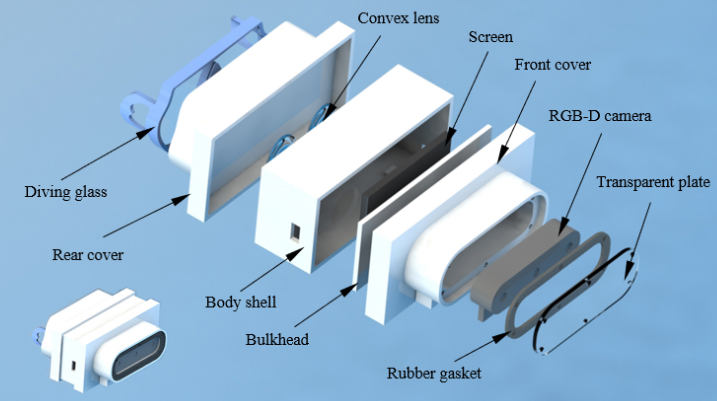
\includegraphics[width=0.8\textwidth]{figures/ch5/headscreen.jpg}
    \caption{相机防护设计}
    \label{img:camera}
\end{figure}

头显的镜片采用聚碳酸酯材料,经过耐冲击和防刮擦处理。
镜框与镜片之间采用液态硅胶封装技术,边缘增加防护垫圈。

(3)散热与气压平衡
嵌入式计算单元的热量通过金属导热片传递至外壳,并通过水体进行散热。
防水舱体内部设计了气压平衡阀,防止外界压力导致设备变形或密封失效。

另外,各部件之间通过防水接头连接,整体结构紧凑,确保在水下环境中的稳定运行。

\section{整体功能设计}
本章设计的水下穿戴式感知系统主要由穿戴式夹克组成,其上集成了防水舱体和水下虚拟现实头显。
该系统能够将直接捕捉视觉数据反馈至头戴式显示器,
通过 Jeston Orin 处理器实时渲染提前处理好的水下三维场景,
并结合手势识别技术实现在水下的全面的交互交互。

\subsection{图像增强与三维重建}
水下可穿戴感知增强系统通过整合第三章提出的水下图像增强算法与第四章的三维重建技术,
将为潜水员提供质量更加高的水下逼真的三维场景。
如图\ref{img:function}所示,
\begin{figure}
    \centering
    \includegraphics[width=0.8\textwidth]{figures/ustc-badge.pdf}
    \caption{系统功能设计}
    \label{img:function}
\end{figure}

\subsection{用户交互与控制}
\subsubsection{手势识别算法}
\subsubsection{交互指令设计}
如表\ref{tab:instruction}所示,系统设计了一套基于手势识别的交互指令,潜水员可以通过手势控制系统的操作。
\begin{table}
    \centering
    \caption{交互指令设计}
    \label{tab:instruction}
    \begin{tabular}{|c|c|}
    \hline
    手势 & 操作 \\
    \hline
    单击 & 选择 \\
    \hline
    双击 & 确认 \\
    \hline
    指向 & 移动 \\
    \hline
    挥动 & 返回 \\
    \hline
    \end{tabular}
\end{table}


